% 页面设置
\documentclass[12pt, a4paper]{article} % 字号:12,纸张:A4
\usepackage[top=2.54cm, bottom=2.54cm, left=3.18cm,right=3.18cm]{geometry} % 页边距设置
% 字体设置
\usepackage[UTF8]{ctex}
\usepackage{fontspec} % 设置字体
%\setCJKmainfont{SimSun}[AutoFakeBold=true, BoldFont={SimHei}, ItalicFont={KaiTi}] % 正文字体
%\setCJKsansfont[AutoFakeBold=3]{KaiTi} % 无衬线字体
%\setCJKmonofont[AutoFakeBold=3]{SimHei} % 等宽字体
\setmainfont{Times New Roman} % 设置主字体为新罗马体
% 文本设置
\usepackage{enumerate} % 支持小标题编号
\linespread{1.5} % 行间距1.5倍
\usepackage{indentfirst}%首段缩进
\setlength{\parindent}{2em} % 首行缩进两字符
\usepackage[hidelinks]{hyperref} % 目录添加超链接
\usepackage{zhnumber} % 章节标题中文显示
\usepackage[cmyk]{xcolor} % 文字彩色显示
% 数学支持
\usepackage{amsmath} % 数学公式支持
\usepackage{amssymb} % 数学符号支持
\usepackage{bm} % 公式加粗
\usepackage{mathrsfs} % 花体字母
\usepackage{yhmath} % 更多的数学符号
% 图片设置
\usepackage{caption} % 插入图片标题
\usepackage{float} % 控制图片位置
\usepackage{subfigure} % 图片并排
\usepackage{booktabs} % 插入表格
% 表格设置
\usepackage{multirow} % 表格自动换行
\usepackage{bigstrut} % 表格间距
\usepackage{rotating} % 表格旋转
\usepackage{tabularx} % 表格宽度
\usepackage{colortbl} % 表格颜色
\usepackage{graphicx} % 表格自动宽度

\title{第二章 \ \ \ 线性模型} % 文章标题
\author{Castor Ye} % 文章作者
\date{} % 文章时间

\begin{document} % 文档从这里开始。
\maketitle % 按照预定的模板把上面那些信息排好。
\newtheorem{definition}{定义}[section]
\newtheorem{theorem}{定理}[section]
\newtheorem{example}{例}[section]
\newtheorem{solution}{题解}
\newtheorem{algorithm}{算法}
\newtheorem{axiom}{公理}
\newtheorem{property}{性质}
\newtheorem{proposition}{命题}
\newtheorem{lemma}{引理}
\newtheorem{corollary}{推论}[section]
\newtheorem{remark}{注解}
\newtheorem{condition}{条件}
\newtheorem{conclusion}{结论}
\newtheorem{assumption}{假设}
\renewcommand{\figurename}{图} % 将图片序号改为图
\renewcommand{\tablename}{表} % 将表格序号改为表
%%%%%%%%%%%%%%%%%%%%%%%%%%%%%%%%%%%%%%%%%%%%%%%%%%%%%%%%%%%%%%%%%%%%%%%
% 文章内容从此开始
\section{基本形式}

给定由 $d$ 个属性描述的示例 $x = (x_1; x_2; \cdots; x_d)$,其中 $x_i$ 是 $x$ 在第 $i$ 个属性上的取值,线性模型(linear model)试图学得一个通过属性的线性组合来进行预测的函数,即:
\begin{equation*}
    f(x) = w_1x_1 + w_2x_2 + \cdots + w_dx_d + b
\end{equation*}

一般用向量形式写成:
\begin{equation*}
    f(x) = w^T x + b
\end{equation*}
其中 $w = (w_1; w_2; \cdots ; w_d)$,$w$ 和 $b$ 学得之后,模型就得以确定。

\section{线性回归}

给定数据集 $D = \{(x_1, y_2), (x_2, y_2), \cdots, (x_m, y_m)\}, x_i = (x_{i1}; x_{i2}; \cdots; x_{id}), y_i \in \mathbb{R}$。“线性回归”(linear regression)试图学得一个线性模型以尽可能准确地预测实值输出标记。例如:根据历年城市 GDP 预测未来 GDP,或者根据历年天气数据预测今年农作物收成等。

对于连续值的属性,一般都可以直接或经过预处理(归一化等)后被学习器所用。但对于离散值,我们可以做以下处理:

\begin{enumerate}[\hspace*{2em} i.]
    \item 若属性间存在“序”(order)关系,可通过连续化将其转化为连续值。例如:身高属性分为“高”“中”“矮”,可转化为数值:$\{1, 0.5, 0\}$。
    \item 若属性间不存在“序”(order)关系,则通常将其转化为向量的形式。例如:性别属性分为“男”“女”,可转化为二维向量:${(1, 0), (0, 1)}$。
\end{enumerate}

线性回归试图学得:
\begin{equation*}
    f(x_i) = wx_i + b, \ \ \text{使得} f(x_i) \simeq y_i
\end{equation*}

为了确定 $w$ 和 $b$,我们可以引入均方误差:
\begin{equation*}
    \begin{array}{*{20}{l}}
        {({w^*},{b^*})}&{ = \mathop {\arg \min }\limits_{(w,b)} \sum\limits_{i = 1}^m {{{(f({x_i}) - {y_i})}^2}} }\\
        {}&{ = \mathop {\arg \min }\limits_{(w,b)} \sum\limits_{i = 1}^m {{{({y_i} - w{x_i} - b)}^2}} }
    \end{array}
\end{equation*}

均方误差有非常好的几何意义,它对应了常用的“欧几里得距离(两点直线距离)”(Euclidean distance)。基于均方误差最小化来进行模型求解的方法称为“最小二乘法”(least square method)。在线性回归中,最小二乘法就是试图找到一条直线,使所有样本到直线上的欧氏距离之和最小。

求解 $w$ 和 $b$ 使 $\displaystyle E_{(w, b)} = \sum_{i = 1}^{m} (y_i - wx_i -b)^2$ 最小化的过程,称为线性回归模型的最小二乘“参数估计”(parameter estimation)。我们可将 $E_{(w, b)}$ 分别对 $w$ 和 $b$ 求导,得到:
\begin{equation*}
    \frac{{\partial {E_{(w,b)}}}}{{\partial w}} = 2\left( {w\sum\limits_{i = 1}^m {x_i^2}  - \sum\limits_{i = 1}^m {({y_i} - b){x_i}} } \right)
\end{equation*}
\begin{equation*}
    \frac{{\partial {E_{(w,b)}}}}{{\partial b}} = 2\left( {mb - \sum\limits_{i = 1}^m {({y_i} - w{x_i})} } \right)
\end{equation*}

令上面两式为零可得到 $w$ 和 $b$ 最优解的闭式(closed-form)解:
\begin{equation*}
    w = \frac{{\sum\limits_{i = 1}^m {{y_i}\left( {{x_i} - \bar x} \right)} }}{{\sum\limits_{i = 1}^m {x_i^2}  - \frac{1}{m}{{\left( {\sum\limits_{i = 1}^m {{x_i}} } \right)}^2}}} \ \ \ b = \frac{1}{m}\sum\limits_{i = 1}^m {({y_i} - w{x_i})}
\end{equation*}
其中 $\displaystyle \bar{x} = \frac{1}{m} \sum_{i = 1}^{m} x_i$,为 $x$ 的均值。

注意:
\begin{enumerate}[\hspace*{2em} i.]
    \item 这里 $E_{(w, b)}$ 是关于 $w$ 和 $b$ 的凸函数,当它关于 $w$ 和 $b$ 的导数均为零时,得到 $w$ 和 $b$ 的最优解。
    \item 对区间 $[a, b]$ 上定义的函数 $f$,若该函数对区间中任意两点 $x_1, x_2$ 均有 $\displaystyle f(\frac{x_1 + x_2}{2}) \le \frac{f(x_1) + f(x_2)}{2}$,则称 $f$ 为区间 $[a, b]$ 上的凸函数。
    \item 对实数集上的函数,可以通过求二阶导数来判别:若二阶导数在区间上非负,则称为凸函数;若二阶导在区间上恒大于零,则为严格凸函数。
\end{enumerate}

更一般的情形是如本节开头的数据集 $D$,样本由 $d$ 个属性描述,此时我们试图学得:
\begin{equation*}
    f(x_i) = w^T x_i + b_i, \ \ \ \text{使得} f(x_i) \simeq y_i
\end{equation*}
这称为“多元线性回归”(multivariate linear regression)。

类似的,可利用最小二乘法来对 $w$ 和 $b$ 进行估计。为便于讨论,我们把 $w$ 和 $b$ 吸收入向量形式 $\hat{w} = (w; b)$,相应的,把数据集 $D$ 表示为一个 $m \times (d + 1)$ 大小的矩阵 $X$,其中每行对应于一个示例,该行前 $d$ 个元素对应于示例的 $d$ 个属性值,最后一个元素恒置为 $1$,即:
\begin{equation*}
    \hat w = (w;b) = {\left[ {\begin{array}{*{20}{c}}
        {{w_1}}&{{w_2}}& \cdots &{{w_d}}&b
    \end{array}} \right]^T}
\end{equation*}
\begin{equation*}
    X = \left[ {\begin{array}{*{20}{c}}
        {{x_{11}}}&{{x_{12}}}& \cdots &{{x_{1d}}}&1\\
        {{x_{21}}}&{{x_{22}}}& \cdots &{{x_{2d}}}&1\\
         \vdots & \vdots & \ddots & \vdots & \vdots \\
        {{x_{m1}}}&{{x_{m2}}}& \cdots &{{x_{md}}}&1
        \end{array}} \right] = \left[ {\begin{array}{*{20}{c}}
        {x_1^T}&1\\
        {x_2^T}&1\\
         \vdots & \vdots \\
        {x_m^T}&1
    \end{array}} \right]
\end{equation*}
\begin{equation*}
    X \cdot \hat w = \left[ {\begin{array}{*{20}{c}}
        {{w_1}{x_{11}} + {w_2}{x_{12}} +  \cdots  + {w_d}{x_{1d}} + b}\\
        {{w_1}{x_{21}} + {w_2}{x_{22}} +  \cdots  + {w_d}{x_{2d}} + b}\\
         \cdots \\
        {{w_1}{x_{m1}} + {w_2}{x_{m2}} +  \cdots  + {w_d}{x_{md}} + b}
        \end{array}} \right] = \left[ {\begin{array}{*{20}{c}}
        {f\left( {{x_1}} \right)}\\
        {f\left( {{x_2}} \right)}\\
         \cdots \\
        {f\left( {{x_m}} \right)}
    \end{array}} \right]
\end{equation*}
再把标记也写成向量形式 $y = (y_1; y_2; \cdots; y_m)$,则有:
\begin{equation*}
    \hat{w}^* = \mathop {\arg \min }\limits_{\hat w} {\left( {y - X\hat w} \right)^T}\left( {y - X\hat w} \right)
\end{equation*}

令 $E_{\hat{w}} = {\left( {y - X\hat w} \right)^T}\left( {y - X\hat w} \right)$,对 $\hat{w}$ 求导得到:
\begin{equation*}
    \frac{{\partial {E_{\hat w}}}}{{\partial \hat w}} = 2{X^T}(X\hat w - y)
\end{equation*}
令上式为零可得 $\hat{w}$ 最优解的闭式解,但由于涉及矩阵逆的计算,比单变量情形要复杂一些,下面做一个简单讨论:

当 $X^TX$ 为满秩矩阵(full-rank matrix)或正定矩阵(positive definite matrix)时,即矩阵行列式不为零时,令上式为零得到:
\begin{equation*}
    \hat{w}^* = (X^TX)^{-1} X^T y
\end{equation*}
其中 $(X^TX)^{-1}$ 是矩阵 $(X^TX)$ 的逆矩阵。令 $\hat{x}_i = (x_i, 1)$,则最终学得的多元线性回归模型为:
\begin{equation*}
    f(\hat{x}_i) = \hat{x}_i^T (X^TX)^{-1} X^Ty
\end{equation*}

对于非满秩矩阵,我们不进行深入。

另一方面,有时候原始的线性回归并不能满足需求。例如:$y$ 并不是线性变化,而是指数变化。此时我们可以采用线性模型来逼近 $y$ 的衍生物,例如 $\ln y$,如下图所示。这就是“对数线性回归”(log-linear regression),它实际上是在试图让 $e^{w^Tx +b}$ 逼近 $y$。

\begin{figure}[H]
    \centering
    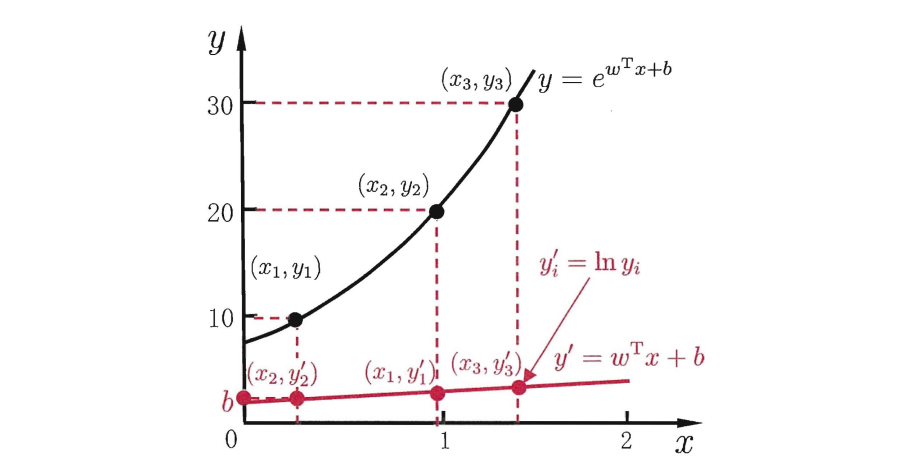
\includegraphics[width=0.8\textwidth]{../img/3-1-对数线性回归示意图.png}
    \caption{对数线性回归示意图}
    \label{fig:对数线性回归示意图}
\end{figure}



\end{document}